
It should be noted that, the meaning of `commonly applied in materials modelling', we implies scenarios where periodic boundary conditions and planewave (or equivalent) basis sets are usually applied in materials simulations, and the dispersion correction schemes discussed below have their equivalent versions being implemented for computations under periodic boundary conditions. However, here we mainly focus on how the dispersion correction schemes were originally developed for molecular systems, in which atom-centred basis sets are used, highlighting how modern dispersion correction scheme account for the chemical environments in an atomistic system. The extension of these from molecular to periodic systems are  technical details on how the total dispersion energies are summed across interacting atomic pairs (and multiplets), that, in our opinion, do not change how the dispersion coefficients are determined by taking into account the local chemical environments, which is the key theoretical aspect we would like to focus here.

\paragraph{\textbf{Grimme's -D3 and -D4 schemes}} The popular -D3 correction was first proposed by \citet{grimme2010consistent} in 2010, where the total dispersion energy is given by the sum of an atom pairwise and triplewise (given in the Axilrod-Teller-Muto form\cite{axilrod1943interaction,muto}) terms:
\begin{equation}\label{eqn:D3}
E_{\mbox{\scriptsize{disp}}}^{{\mbox{\scriptsize{D3}}}}=-\sum_{AB}\sum_{n=6,8}s_n \frac{C_n^{\mbox{\scriptsize{AB}}}}{R^n}f_{\mbox{\scriptsize{damp}}}^{(n)}(R)-\sum_{ABC}s_9 \frac{C_{9}^{\mbox{\scriptsize{ABC}}}(3\cos\theta_a \cos\theta_b\cos\theta_c +1)}{(R_{AB}R_{AC}R_{BC})^3}f_{\mbox{\scriptsize{damp}}}^{(9)}(\bar{R}_{ABC}).
\end{equation}
Here, the leading $C_6^{\mbox{\scriptsize{AB}}}$ coefficients are calculated from its corresponding reference value $C_{6,\mbox{\scriptsize{ref}}}^{\mbox{\scriptsize{AB}}}$ determined from the polarisabilities of model hydrides A$_m$H$_n$ and B$_k$H$_l$ systems using a modified version of \cref{eq:casimir_eq}:
\begin{equation}\label{eq:d3-casimir-eq}
C_{6,\mbox{\scriptsize{ref}}}^{\mbox{\scriptsize{AB}}}(\mbox{CN}^A,\mbox{CN}^{B})=\frac{3}{\pi}\int_0^\infty\frac{1}{m}\left[\alpha^{A_m H_n}(i\omega)-\frac{n}{2}\alpha^{H_2}(i\omega)\right]\times\frac{1}{k}\left[\alpha^{B_k H_l}(i\omega)-\frac{l}{2}\alpha^{H_2}(i\omega)\right]\mbox{d}\omega,
\end{equation}
in which CN for atom A in the reference molecule is given by:
\begin{equation}\label{eq:D3_coord_nummer}
\mbox{CN}^A=\sum_{B\neq A}^{N_{atoms}}\left\{1+\exp\left[-16\frac{4(R_{A,\mbox{\scriptsize{cov}}}+R_{B,\mbox{\scriptsize{cov}}})}{3R_{AB}-1}\right]\right\}^{-1},
\end{equation}
where $R_{A,\mbox{\scriptsize{cov}}}$ is the covalent radius of element A. As illustrated in \cref{fig:grimme_dispersions}(a), the inclusion of the CN effectively reduces the magnitude of the atomic $C_6$ coefficients for bare atoms to those with a high CN (hence less exposed electron density). With the precomputed pairwise $C_{6,\mbox{\scriptsize{ref}}}^{\mbox{\scriptsize{AB}}}$, in the actual D3 calculation for the target system, the pairwise atom $C_{6}^{\mbox{\scriptsize{AB}}}$ is further calculated as the Gaussian average of the precomputed values:
\begin{equation}\label{eq:actual_c6_grimme}
C_{6}^{\mbox{\scriptsize{AB}}}(\mbox{CN}^A,\mbox{CN}^{B})=\frac{\sum_i^{N_A}\sum_j^{N_B}C_{6,\mbox{\scriptsize{ref}}}^{\mbox{\scriptsize{AB}}}(\mbox{CN}^A,\mbox{CN}^{B})L_{ij}}{\sum_i^{N_A}\sum_j^{N_B}L_{ij}},
\end{equation}
with $L_{ij}=\exp\left\{-4[(\mbox{CN}^A-\mbox{CN}_i^A)^2+(\mbox{CN}^B-\mbox{CN}_i^B)^2] \right\}$. The next order $C_8^{\mbox{\scriptsize{AB}}}$ take into account the dipole-quadrupole contribution to the dispersion interaction, which is computed recursively as $C_8^{\mbox{\scriptsize{AB}}}=3C_6^{\mbox{\scriptsize{AB}}}\sqrt{Q_A Q_B}$ with $Q_{A}=\sqrt{Z_A}\frac{\langle r_A^4\rangle}{\langle r_A^2\rangle}$ where $Z_A$ is the atomic number of element A and $\langle r_A^4\rangle$ and $\langle r_A^2\rangle$ are multipole-type expectation values
derived from atomic densities. The scaling factor $s_6$ is typically set to unity and $s_8$ term is used to absorb higher order multipolar terms into the $R^{-8}$ term. Finally, the three-body dispersion coefficient is approximated as $C_{9}^{\mbox{\scriptsize{ABC}}}\approx-\sqrt{C_{6}^{\mbox{\scriptsize{AB}}}C_{6}^{\mbox{\scriptsize{AC}}}C_{6}^{\mbox{\scriptsize{BC}}}}$.

\begin{figure}[tb]
    \centering
    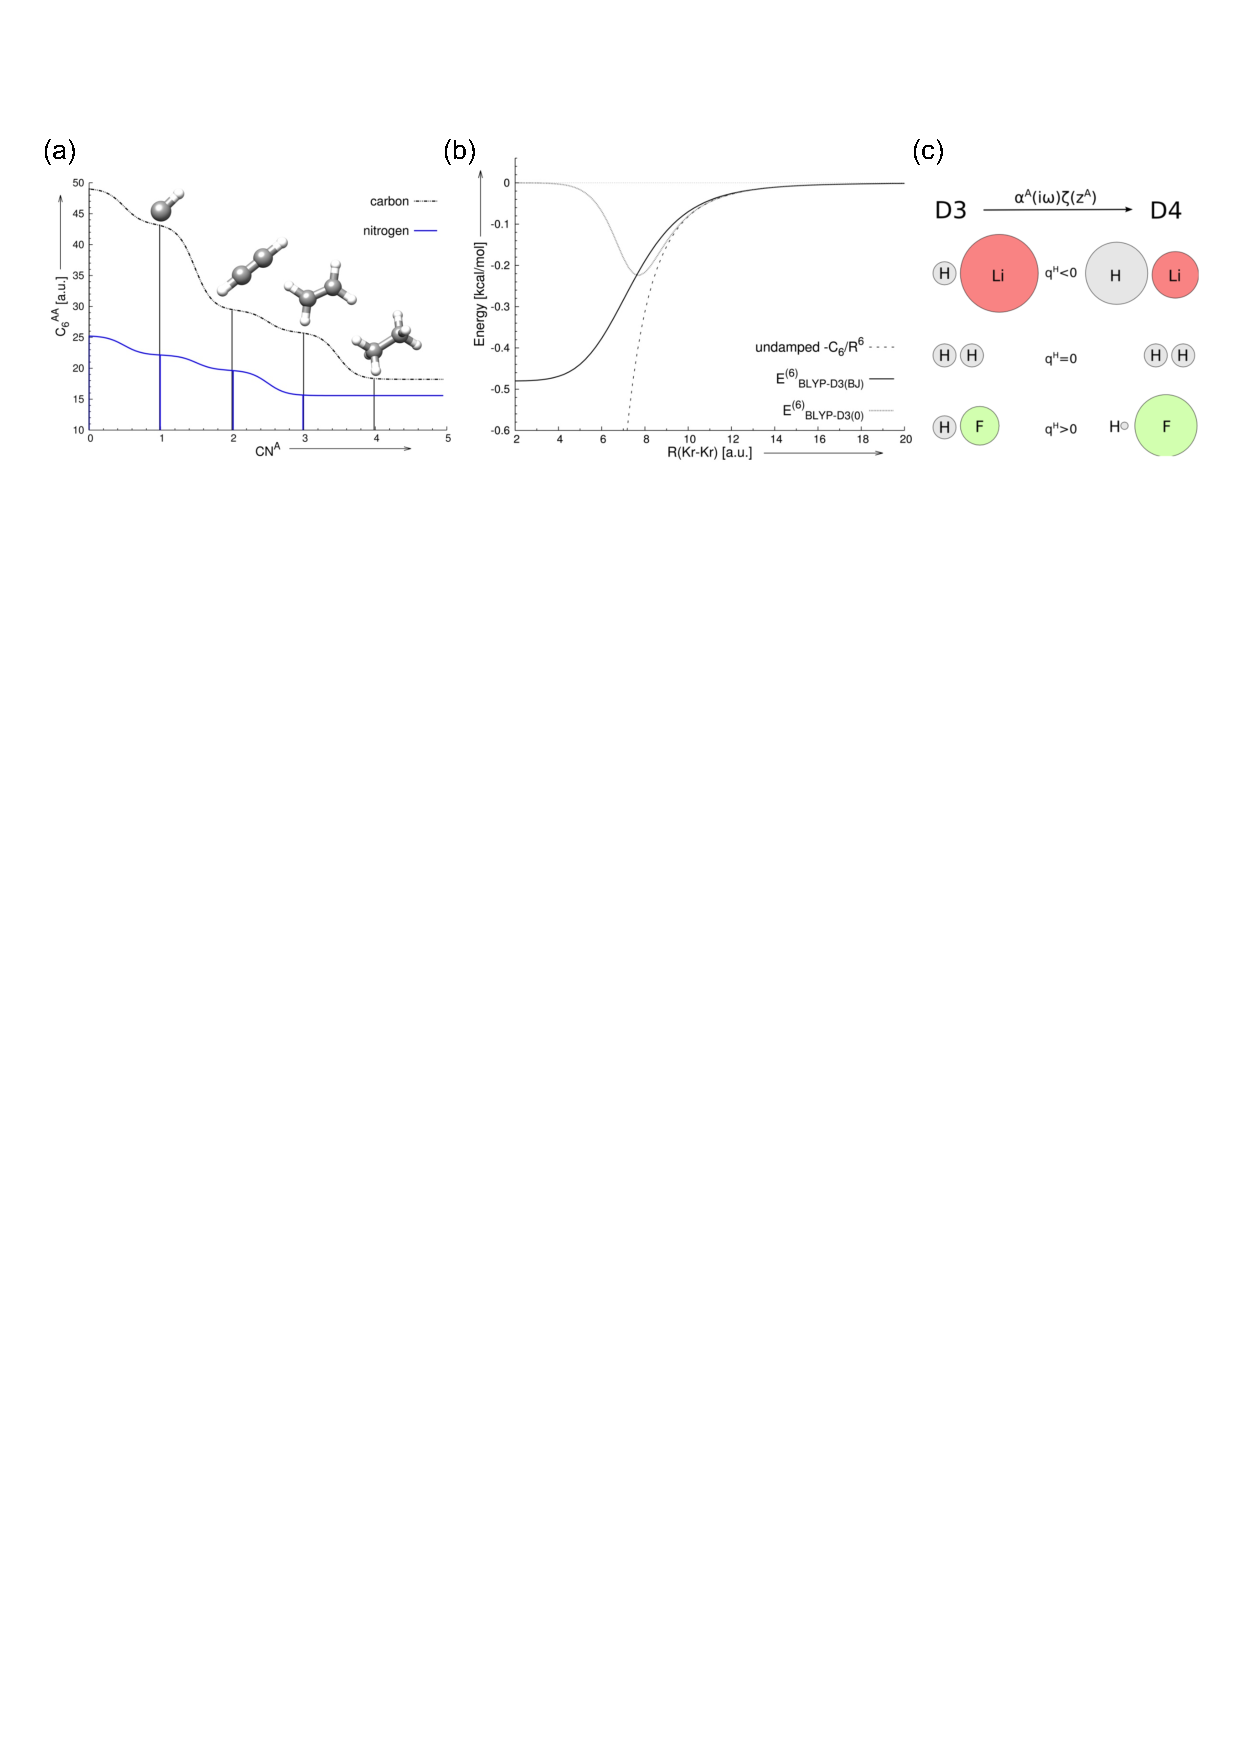
\includegraphics[width=\linewidth]{grimme_dispersions.pdf}
    \caption{Key features in Grimme's $-$D3 and $-$D4 dispersion correction schemes. (a) CN-dependent atom pairwise dispersion coefficient for homoatomic pairs $C_{6}^{AA}$ as a function of the coordination number CN$^{A}$. The reference points $C_{6,ref}^{AA}$ are drawn as vertical sticks in the respective colours (black for carbon, blue for nitrogen). For carbon, the structures of CH, ethyne, ethene, and ethane (corresponding to the coordination numbers 1-4) are depicted as well. (b) Different D3 damping schemes for the $E_{\mbox{\scriptsize{disp}}}^{(0)}$ contribution of the Kr-Kr dispersion energy. For D3(BJ) (solid black) and D3(0) (dotted gray), the curves are given using the damping parameters for the BLYP functional. The undamped $-C_{6}/R^{6}$ contribution is given for comparison (dashed black). [Adapted from \citet{grimme2016dispersion}] (c) Schematic representation of the $\zeta$-functionality which rescales atomic polarisabilities based on input Mulliken charges $q$ in the $-$D4 model. The left side shows the standard partitioning of atomic polarisabilities in D3. On the right side, the scaled atomic polarisabilities are shown. The depicted radii of the atoms directly correspond to the calculated atomic $C_{6}^{AA}$ coefficients. [Adapted from \citet{caldeweyher2017extension}]}
    \label{fig:grimme_dispersions}  
\end{figure} 


Furthermore, as shown in \cref{fig:grimme_dispersions}(b), the undamped dispersion energy $-C_6/R^6$ decays to negative infinity at small interatomic distance, that can lead to the unphysical behaviours of atoms collapsing into each other when combined with standard DFT calculations. This problem can be overcome by including an additional damping function $f_{\mbox{\scriptsize{damp}}}^{(n)}(R)$. For the -D3 scheme, both zero damping\cite{chai2008long} (which brings the dispersion energy to zero at zero interatomic separation) and Becke-Johnson (BJ)\cite{johnson2005post,grimme2011effect} damping are available, with the later being the default choice for the -D3 scheme [dubbed as -D3(BJ)].

In 2017, the -D3 model is extended to its new version, termed as the -D4 model.\cite{caldeweyher2017extension,caldeweyher2019generally} The significant improvement in the newer model [\cref{fig:grimme_dispersions}(c)] is the scaling of the polarisabilities [\emph{c.f} \cref{eq:d3-casimir-eq}] based on the atomic charge $\alpha^{A}(i\omega)\to\alpha^{A}(i\omega)\zeta(Z^A)$ computed in the target molecular environment. Consequently, the dispersion coefficient can no longer be precomputed and the Casimir-Polder integral must be evaluated on-the-fly to obtain the atomic dispersion coefficients that can more accurately account for the electrostatic environment of each atom in specific molecules.

\paragraph{\textbf{The Tkatchenko-Scheffler (TS) models}} In 2009, \citet{tkatchenko2009accurate} put forward an atom pairwise dispersion correction scheme that is similar to the -D3 correction, except that the atom polarisability $\alpha_A$ and the $C_6^{AA}$ dispersion coefficients are density-dependent by scaling them from their free-atom values as:
\begin{equation}\label{eq:TS_pol_scaling}
    \alpha_A=v_A\alpha_{\mbox{\scriptsize{free}}}^A\qquad\mbox{and}\qquad C_6^{AA}=v_A^2C_{6,{\mbox{\scriptsize{free}}}}^{AA},
\end{equation}
in which the scaling coefficient is computed based on the Hirshfeld charge density partition scheme\cite{hirshfeld1977bonded} as
\begin{equation}\label{eq:hirshfeld}
v_A=\frac{\displaystyle{\int} r^3 w_A(\bm{r})\rho(\bm{r})\mbox{d}^3\bm{r}}{\displaystyle{\int} r^3 \rho^{\mbox{\scriptsize{free}}}_{A}(\bm{r})\mbox{d}^3\bm{r}}, \qquad \mbox{with}\qquad w_A(\bm{r})=\frac{\rho^{\mbox{\scriptsize{free}}}_{A}(\bm{r})}{\sum_B \rho^{\mbox{\scriptsize{free}}}_{B}(\bm{r})}.
\end{equation}

Subsequently, the TS dispersion model is extended beyond pairwise additivity to account for the dispersion interaction that arises from the collective fluctuation of electron densities in the interacting molecules, thus reflecting the intrinsic many-body effects behind dispersion interactions\cite{tkatchenko2012accurate,tkatchenko2013interatomic} [also see \cref{sect:polarisable_FF} for detailed discussion]. This means that the atomic polarisabilities and dispersion coefficients for an atom in the target molecular system will be affected by those of the other atoms present in the same system. To account for such an effect, the many-body TS model represents all atoms in the system as a collection of quantum harmonic oscillators, which are able to interact with each others and alter the dynamic electronic polarisability of every atom. As such, 
the imaginary frequency dipole polarisability of any atom $p$ needs to be computed self-consistently from the polarisabilities of all other atoms $q\neq p$ in the system as
\begin{equation}\label{eq:SCS_polarisation}
\alpha_{p}^{\mbox{\scriptsize{SCS}}}(i\omega)=\alpha_{p}^{\mbox{\scriptsize{TS}}}(i\omega)+\alpha_{p}^{\mbox{\scriptsize{TS}}}(i\omega)\sum_{p\neq q}\hat{\mathcal{T}}_{pq}\alpha_{q}^{\mbox{\scriptsize{SCS}}}(i\omega),
\end{equation}
 in which $\hat{\mathcal{T}}_{pq}$ is the dipole-dipole interaction tensor. From here, the many-body dispersion energy is then computed using the coupled fluctuating dipole model by diagonalising the coupling matrix of the fluctuating dipole moments.

An other extension to the many-body TS model is the fractionally ionic approach (FIA)\cite{gould2016fractionally} to properly account for the ionic charge and volumes in fully ionic systems that can differ significantly from molecular systems. Here, the frequency-dependent atomic dipole polarisability model employed for a system with non-integer electron number $N$ is a linear interpolation of the polarisabilities for system with $M=\lfloor N \rfloor$ and $M+1$ electrons. Compared to the standard -D3 and TS dispersion correction scheme (MAE $\sim 1.5-1.8$ meV/\AA) , the FIA (MAE $\sim 0.9$ meV/\AA) provides notable improvements in the binding energies of ionic 2D materials.\cite{tawfik2018evaluation} This clearly shows that practitioners of computational materials studies should be more cautious in using `generally applicable' methodologies, particularly be aware of the assumption(s) adapted behind the developed method.

\paragraph{\textbf{The exchange-dipole moment (XDM) model}}
The XDM model is the density-dependent dispersion correction model proposed by Becke and Johnson in 2005.\cite{johnson2005post,becke2005density,becke2005exchange,johnson2006post,becke2007exchange,otero2013many} The starting point of the XDM model is to reformulate the exact exchange interactions [\cref{eq:exchange_HF_DFT}] as (spin-dependent, labelled with $\sigma=\uparrow$ and $\downarrow$) a localised electron density interacting with a nonlocal exchange hole $h_{X\sigma}(\bm{r},\bm{r}^\prime)$ as
\begin{equation}\label{eq:exchange_interaction_hole_form}
    E_{x}=\frac{1}{2}\sum_{\sigma}\int \mbox{d}\bm{r}\int\mbox{d}\bm{r}^\prime \rho_\sigma (\bm{r})\frac{h_{X\sigma}(\bm{r},\bm{r}^\prime)}{|\bm{r}-\bm{r}^\prime|}.
\end{equation}
whereby in Kohn-Sham DFT, the exchange hole can be computed as
\begin{equation}\label{eq:exchange_hole}
h_{X\sigma}(\bm{r},\bm{r}^\prime)=-\frac{1}{\rho_\sigma(\bm{r})}\sum_{ij} \phi_{i\sigma}(\bm{r}) \phi_{j\sigma}(\bm{r}) \phi_{i\sigma}(\bm{r}^\prime) \phi_{j\sigma}(\bm{r}^\prime),
\end{equation}
which involves the summation over the occupied spin-orbitals ($\psi_{i\sigma}$). Typically, the exchange hole is not spherically symmetry around the electron, leading to a non-vanishing exchange (hole) dipole moment and analogously higher order exchange hole multipoles, thus one can imagine the dispersion interaction arises from the instantaneous interaction between the exchange and induced dipole (and multipole) moments of two fragments A and B (which, in the XDM model, are defined using the Hirshfeld partitioning scheme as in \cref{eq:hirshfeld}). The exchange hole dipole moment, in this case, is
\begin{equation}\label{eq:exchange_dipole_moment}
\bm{\mu}_{X\sigma}(\bm{r})=\int \bm{r}^\prime h_{X\sigma}(\bm{r},\bm{r}^\prime)\mbox{d}\bm{r}^\prime -\bm{r}.
\end{equation}
From here, the square of the $l$-pole operator can be calculated as:
\begin{equation}\label{eq:XDM_l_pole_moment}
\langle M_l^2\rangle_A=\sum_\sigma\int \rho_\sigma(\bm{r})[r_A^l -(r_A-\mu_{X\sigma}(\bm{r}))^l]^2\mbox{d}\bm{r},
\end{equation}
which allows the two-body dispersion coefficients to be obtained as:
\begin{align}
    C_6^{\mbox{\scriptsize{AB}}}&=\frac{\alpha_A\alpha_B\langle M_{1}^2\rangle_A\langle M_{1}^2\rangle_B}{\alpha_B \langle M_{1}^2\rangle_A+\alpha_A \langle M_{1}^2\rangle_B}, \label{eq:XDM_C6}\\
    C_8^{\mbox{\scriptsize{AB}}}&=\frac{3}{2}\frac{\alpha_A \alpha_B (\langle M_{1}^2\rangle_A \langle M_{2}^2\rangle_B+ \langle M_{2}^2\rangle_A\langle M_{1}^2\rangle_B)}{\alpha_B \langle M_{1}^2\rangle_A+\alpha_A \langle M_{1}^2\rangle_B}, \label{eq:XDM_C8}\\
    C_{10}^{\mbox{\scriptsize{AB}}}&=2\frac{\alpha_A \alpha_B (\langle M_{1}^2\rangle_A \langle M_{3}^2\rangle_B+ \langle M_{3}^2\rangle_A\langle M_{1}^2\rangle_B)}{\alpha_B \langle M_{1}^2\rangle_A+\alpha_A \langle M_{1}^2\rangle_B}+\frac{21}{5}\frac{\alpha_A\alpha_B\langle M_{2}^2\rangle_A\langle M_{2}^2\rangle_B}{\alpha_B \langle M_{1}^2\rangle_A+\alpha_A \langle M_{1}^2\rangle_B}, \label{eq:XDM_C10}
 \end{align}
in which $\alpha$ are the atomic polarisability determined as in \cref{eq:TS_pol_scaling}. With these, the dispersion correction to the DFT energy takes the form of 
\begin{equation}\label{eq:XDM_disp_energy}
E_{\mbox{\scriptsize{disp}}}^{\mbox{\scriptsize{XDM}}}=-\sum_{AB}\sum_{n=6,8,10}\frac{C_n^{\mbox{\scriptsize{AB}}}}{R^n}f_{\mbox{\scriptsize{damp}}}^{(n)}(R),
\end{equation}
where $f_{\mbox{\scriptsize{damp}}}^{(n)}(R)$ is the Becke-Johnson damping function. Extension of the XDM model to include the three-body Axilrod-Teller-Muto term had also been established,\cite{otero2013many} but it is not used by default in XDM as the dispersion energy vary significantly with the underlying choice of the damping function 



\paragraph{V\textbf{ydrov and Van Voorhis functionals}} Instead of applying a \emph{post hoc} correction of the dispersion interaction energy to the DFT energy, alternative approach that seeks to construct nonlocal correlation functionals that use electron density as the direct input, and an integration kernel $\Phi(\bm{r},\bm{r}^\prime)$ that correlates the electron densities at two electron coordinates:
\begin{equation}\label{eq:nonlocal_disp_corr_kernel}
E_{c}^{\mbox{\scriptsize{NL}}}=\frac{1}{2}\int \mbox{d}\bm{r} \int \mbox{d}\bm{r}^\prime\rho(\bm{r})\Phi(\bm{r},\bm{r}^\prime) \rho(\bm{r}^\prime) .
\end{equation}
Along this venue of method development,\cite{grafenstein2009efficient,dion2004van,lee2010higher,vydrov2009improving,vydrov2009nonlocal,vydrov2010nonlocal} the VV10 functional constructed by \citet{vydrov2010nonlocal} in 2010 represents the one with the simplest functional form and the best accuracy for molecular systems. Here, the correlation kernel is introduced \emph{ad hoc} based on author's experience:
\begin{equation}\label{eq:vv10_kernel}
\Phi(\bm{r},\bm{r}^\prime)=-\frac{3}{2gg^\prime(g+g^\prime)}, 
\end{equation}
with $g=\omega_0(\bm{r})|\bm{r}-\bm{r}^\prime|^2+\kappa(\bm{r})$ and $g^\prime=\omega_0(\bm{r}^\prime)|\bm{r}-\bm{r}^\prime|^2+\kappa(\bm{r}^\prime)$. Here, $\omega_0(\bm{r})$ is related to the local plasma frequency  $\omega_p
(\bm{r})=\sqrt{4\pi\rho(\bm{r})}$ and local band gap $\omega_g(\bm{r})=\sqrt{C\left\vert\nabla \rho(\bm{r})/\rho(\bm{r})\right\vert}$ 
(with $C$ being the adjustable parameter) as $\omega_0(\bm{r})=\sqrt{\omega_g^2(\bm{r})+\omega_p^{2}(\bm{r})/3}$, and the other component in $g$ is $\kappa(\bm{r})=b[3\pi\rho(\bm{r})^{1/3}]/\omega_{p}(\bm{r})$, in which $b$ is a parameter can be adjusted\cite{hujo2011performance} to different standard density functionals that is similar to the DFT-D3 schemes. Finally, a constant multiplied by the number of electrons in the system is included additionally in the correlation kernel to ensure that the long-range correlation energy vanishes in the uniform electron gas limit. Another important aspect of this particular nonlocal density functional is that there exists a self-consistent implementation of the functional,\cite{vydrov2010implementation} which enables one to study the influence of dispersion interactions on the topology of  electron  densities, otherwise not possible from \emph{post hoc} dispersion-corrected DFT methods.